%----------------------------------------------------------------------------------------
%	Header stuff that doesn't really matter...
%----------------------------------------------------------------------------------------
\documentclass[paper=letter, fontsize=11pt]{scrartcl}
\usepackage[T1]{fontenc}
\usepackage{fourier}
\usepackage[english]{babel}
\usepackage{amsmath,amsfonts,amsthm}
\usepackage{caption}
\usepackage{sectsty}
\usepackage{graphicx}
\usepackage{float}
\allsectionsfont{\normalfont\sffamily\bfseries}
\usepackage{fancyhdr}
\fancyhead[R]{Phil Crumm 804-005-575 | Connor Proctor 703-999-284}
\fancyfoot[L]{}
\fancyfoot[C]{}
\fancyfoot[R]{\thepage}
\renewcommand{\headrulewidth}{0pt}
\renewcommand{\footrulewidth}{0pt}
\setlength{\headheight}{13.6pt}

%----------------------------------------------------------------------------------------
%	Title area
%----------------------------------------------------------------------------------------

\newcommand{\horrule}[1]{\rule{\linewidth}{#1}}

\title{	
\normalfont \normalsize 
\textsc{University of California, Los Angeles} \\ [25pt]
\horrule{0.5pt} \\[0.4cm]
\Large Computer Science M152A - Digital Design Lab \\
\horrule{2pt} \\[0.5cm]
}

\author{Connor Proctor \\* 703-999-284 \\* Phillip Crumm \\*804-005-575 \\* \\*Lab 4: Stopwatch}

\date{\normalsize February 27, 2014}
\usepackage[parfill]{parskip}
\begin{document}

\clearpage\maketitle
\thispagestyle{empty}
\pagebreak

%----------------------------------------------------------------------------------------
%	The body
%----------------------------------------------------------------------------------------

\section{Objective}
This laboratory's purpose is to use the Xilinx ISE program and the FPGA to design, implement, and test a reasonably accurate one-hour stopwatch.

\section{Overall Design}
We use the 100MHz clock on the FPGA board to implement a 1Hz clock to drive our stopwatch. We step down the 100MHz signal as described in the laboratory manual. We use this signal to drive a zero-indexed sixty-counter: this is used directly to display the number of elapsed seconds. We use the TC bit of this sixty-counter (HI only when the counter reaches 60) to control the clock on a second sixty-counter: this is used to count elapsed minutes. These counters are attached directly to a seven-segment decoder to illuminate the FGPA's displays.

The FPGA accepts only one seven-segment input. We use a 625Hz output from our clock to cycle between the four seven-segment enables on the FPGA, and a multiplixer to select the appropriate display for output.

Additional complexity is introduced with the reset and adjust functionality. Reset is implemented trivially by attaching directly to the reset bits on the sixty-counters. Adjust is implemented though connection to the CLK input on sixty-counter, which will be described further.

\begin{figure}[H]
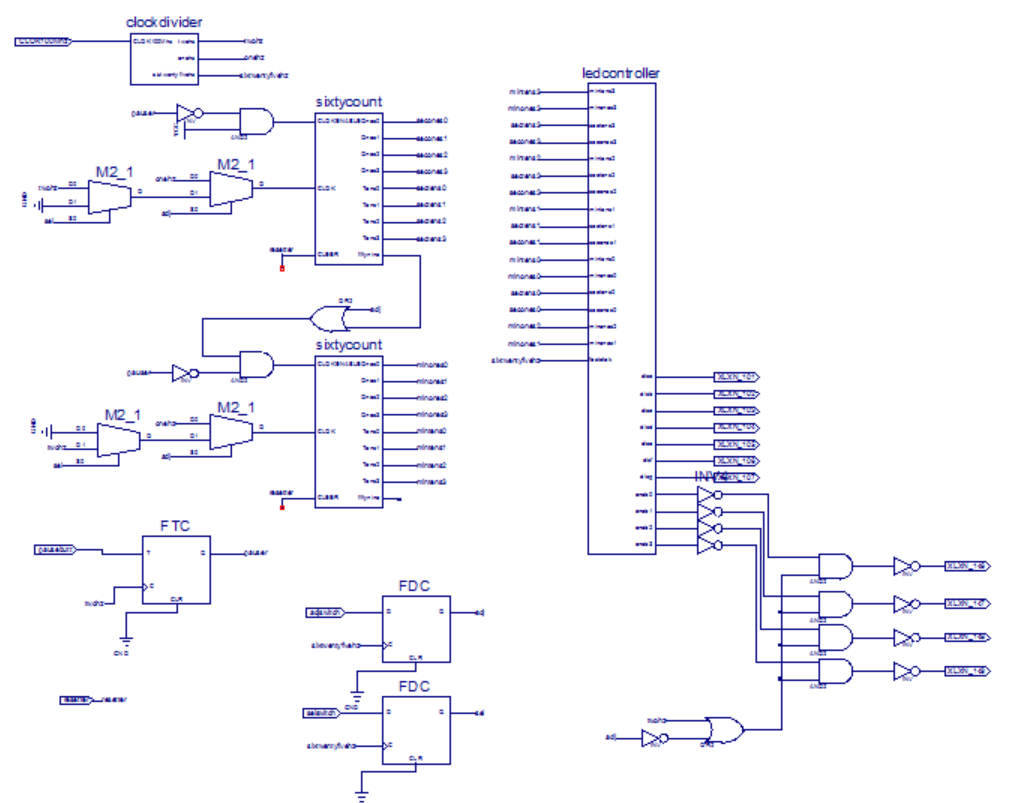
\includegraphics[height=120mm]{wholething.PNG}
\centering
\caption{Implementation Overview}
\label{overflow}
\end{figure}

\subsection{Clock Reducer}
The clock reducer is implemented as described in the laboratory manual. Using the FPGA's single 100MHz clock, we chain together two five-thousand counters. We then attach these counters to chains of flip-flops to further divide by two. Using this technique, we generate 1Hz, 2Hz, and 625Hz clock signals for later use.

\begin{figure}[H]
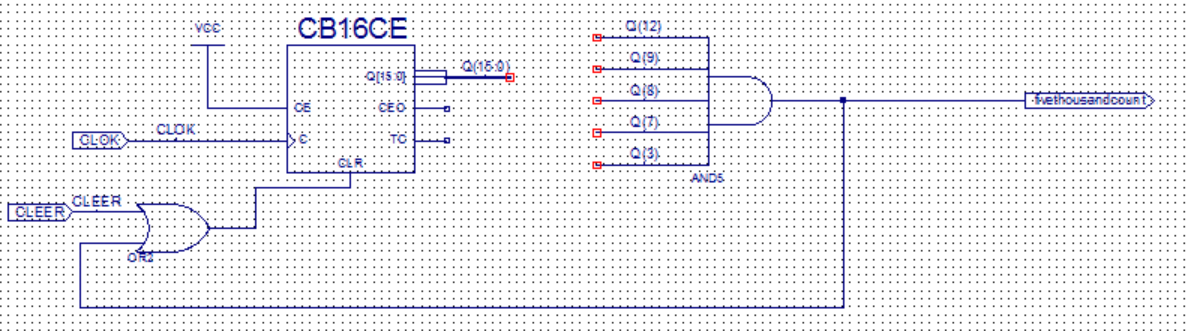
\includegraphics[height=120mm]{countfivethousand.PNG}
\centering
\caption{Clock Reducer}
\label{overflow}
\end{figure}

\subsection{Sixty Counter}
Our sixty-counters are implemented as two decade counters. When the first decade counter reaches 10, it resets itself to zero and fires the clock enable bit on the second decade counter. When this decade counter reaches 6, it sets its TC to high and rolls over similarly. Together, these two counters reliably count to 60 using a 1Hz clock input.

\begin{figure}[H]
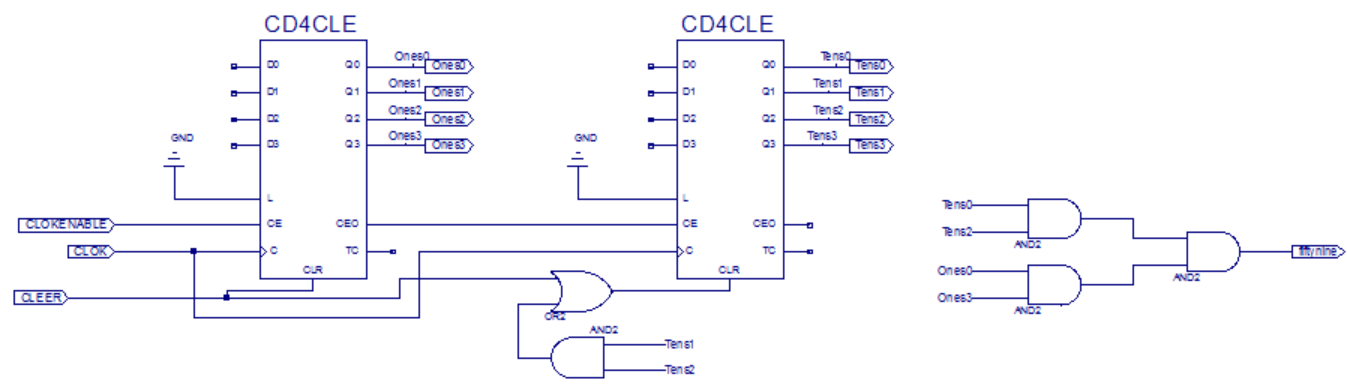
\includegraphics[height=120mm]{decadecounter.PNG}
\centering
\caption{Decade Counterr}
\label{overflow}
\end{figure}

\subsection{Reset}
The debounced reset button is connected directly to the reset input for each sixty-counter.

\subsection{Adjust}
The adjust input is implemented as two switches. The first switch enables the adjust functionality: the second adjusts minutes instead of seconds.

This funcionality is implemented through use of a multi-plexer. When adjust is enabled and the minute switch is off, our multiplexer stops clock pulses for the minutes counter and sets the CLK input on the seconds counter to 2HZ, effectively doubling the clocking speed. Note that this means that any roll-over will NOT cause the minutes timer to increment.

When the minutes switch is enabled, functionality is reversed: the CLK is grounded (stopped) for the seconds counter, and set to 2Hz for the minutes counter. When these switches are set to off, functionality resumes as normal.

\subsection{LED Controller}
The LED controller accepts the input for each clock and decodes the input (zero to 59) into a proper two-digit seven-segment code using schematic implementation of switching expressions we worked out manually.

The LED controller also takes as input the 625Hz clock signal. This is a refresh signal: on each clock cycle, we increment a four-counter which is used to select the proper seven-segment display to activate. In this manner, we "scan" across the seven segment display, illuminating each digit briefly. As the human eye cannot detect refresh rates above 35Hz or so, this means that all four displays appear to be persistently illuminated.

\begin{figure}[H]
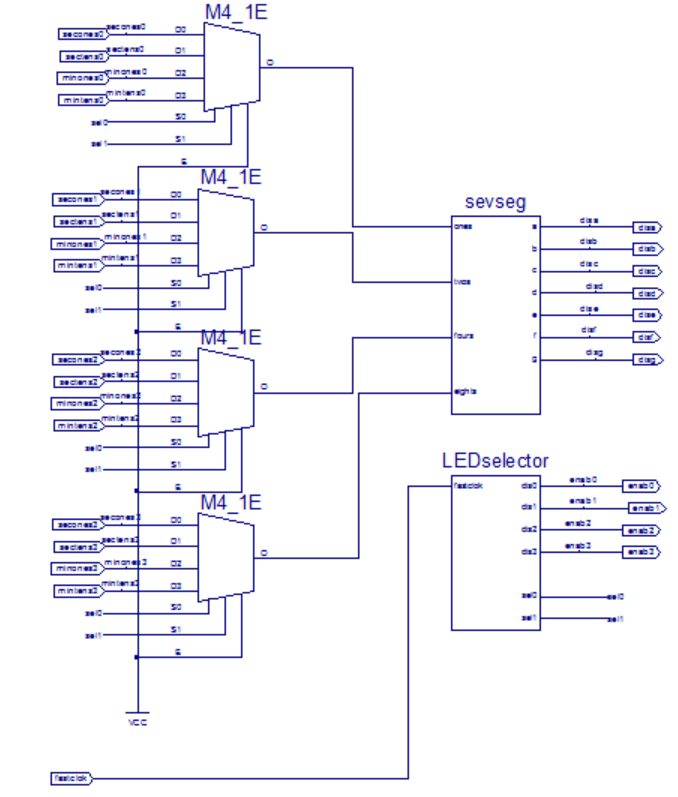
\includegraphics[height=120mm]{led.PNG}
\centering
\caption{LED Controller}
\label{overflow}
\end{figure}

\subsection{Implementation Difficulties}
The bulk of our trouble was in constructing the initial clock. We initially attempted to design our own clock step-down mechanism (rather than using two five-thousand counters), and found that chaining multiple counters created a very noisy signal. After we re-read the lab and stuck to the suggested design, these problems were resolved.

Most other difficulty was found in the confusion of active HI and active LO, which was resolved through trial and error.

%----------------------------------------------------------------------------------------

\end{document}